\documentclass[border=8pt]{standalone}
\usepackage{tikz,xfp}
\newcommand*{\drawtower}[2]{
    \foreach \i[
        count = \cnt from 0,
        evaluate = \i as \k using int(#1-\i),
        evaluate = \i as \l using int(#1-\i+1),
    ] in {1,...,#1}{
        \node at (\fpeval{{#1}/2},-.5) {\textbf{Fig.#2}};
        \ifodd\l
            \filldraw[white] (60:\cnt) -- ++(\l,0) -- ++(120:\l) -- cycle;
        \else
            \filldraw[gray!80] (60:\cnt) -- ++(\l,0) -- ++(120:\l) -- cycle;
        \fi
        \foreach \j[parse=true] in {0,...,\k}{
            \draw[line join=round,shift={(60:\cnt)},shift={(\j,0)},black] (0,0) -- (60:1) -- (1,0) --cycle;}
    }
}
\begin{document}
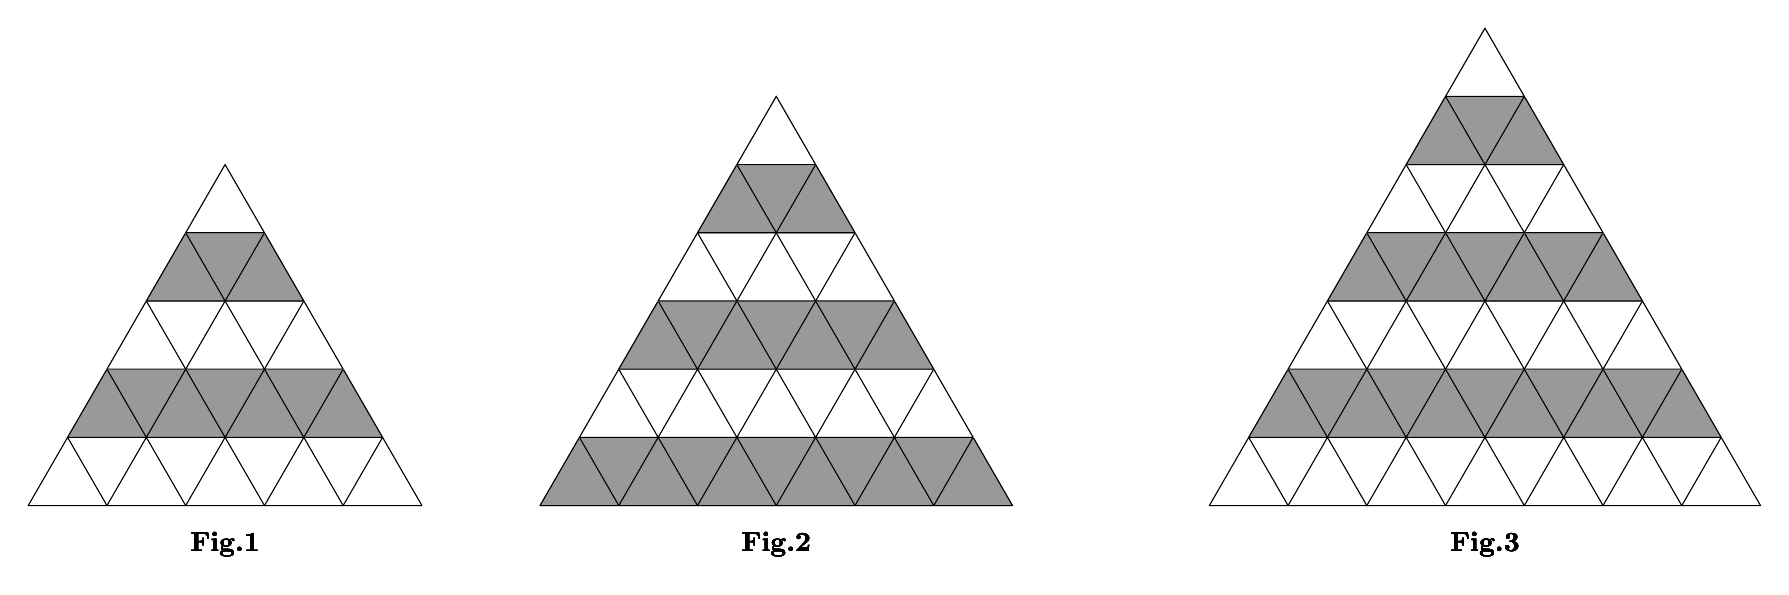
\begin{tikzpicture}
    \drawtower{5}{1}
    \begin{scope}[xshift=6.5cm]
        \drawtower{6}{2}
    \end{scope}
    \begin{scope}[xshift=15cm]
        \drawtower{7}{3}
    \end{scope}
\end{tikzpicture}
\end{document}